\documentclass[tikz,border=2pt]{standalone}
\usepackage{amsmath}
\usetikzlibrary{arrows.meta,calc}
\begin{document}
% Orthonormal basis q_1 = (1,1)^T/sqrt2, q_2 = (1,-1)^T/sqrt2 of R^2 (unit length, perpendicular).
% For x = (3,1)^T the coordinates are x.q_1 = 2 sqrt2 and x.q_2 = sqrt2: the feet of the perpendiculars
% from x onto the two lines are 2 sqrt2 q_1 = (2,2)^T and sqrt2 q_2 = (1,-1)^T, and they add up to x.
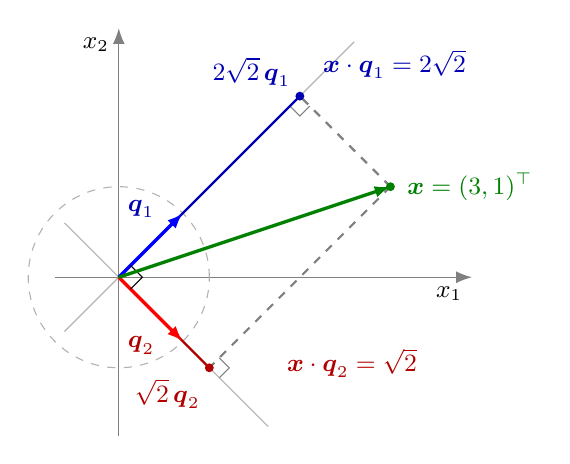
\begin{tikzpicture}[font=\small, >={Latex[length=2mm]}, x=1.15cm, y=1.15cm]
  % standard axes
  \draw[->, gray] (-0.7,0) -- (3.9,0) node[below left, black] {$x_1$};
  \draw[->, gray] (0,-1.75) -- (0,2.75) node[below left, black] {$x_2$};
  % lines through q_1 and q_2
  \draw[gray!60, thin] (-0.6,-0.6) -- (2.6,2.6);
  \draw[gray!60, thin] (-0.6,0.6) -- (1.65,-1.65);
  % unit circle
  \draw[gray!60, thin, dashed] (0,0) circle (1);
  % perpendiculars from x to the two lines
  \draw[gray, thick, dashed] (3,1) -- (2,2);
  \draw[gray, thick, dashed] (3,1) -- (1,-1);
  \draw[gray] ($(2,2)+(0.11,-0.11)$) -- ++(-0.11,-0.11) -- ++(-0.11,0.11);
  \draw[gray] ($(1,-1)+(0.11,0.11)$) -- ++(0.11,-0.11) -- ++(-0.11,-0.11);
  % coordinates along the lines
  \draw[blue!70!black, thick] (0,0) -- (2,2);
  \draw[red!70!black, thick] (0,0) -- (1,-1);
  \fill[blue!70!black] (2,2) circle (1.6pt);
  \fill[red!70!black] (1,-1) circle (1.6pt);
  \node[blue!70!black, anchor=south east] at (2,2) {$2\sqrt{2}\,\boldsymbol{q}_1$};
  \node[red!70!black, anchor=north east] at (1,-1.02) {$\sqrt{2}\,\boldsymbol{q}_2$};
  % basis vectors
  \draw[->, blue, very thick] (0,0) -- (0.7071,0.7071);
  \draw[->, red, very thick] (0,0) -- (0.7071,-0.7071);
  \node[blue!70!black, anchor=south east] at (0.5,0.55) {$\boldsymbol{q}_1$};
  \node[red!70!black, anchor=north east] at (0.5,-0.55) {$\boldsymbol{q}_2$};
  \draw[black] (0.13,0.13) -- (0.26,0) -- (0.13,-0.13);
  % the vector x
  \draw[->, green!50!black, very thick] (0,0) -- (3,1);
  \fill[green!50!black] (3,1) circle (1.6pt);
  \node[green!50!black, anchor=west] at (3.08,1) {$\boldsymbol{x}=(3,1)^{\top}$};
  % coordinate values
  \node[blue!70!black, anchor=west] at (2.15,2.35) {$\boldsymbol{x}\cdot\boldsymbol{q}_1=2\sqrt{2}$};
  \node[red!70!black, anchor=west] at (1.75,-0.95) {$\boldsymbol{x}\cdot\boldsymbol{q}_2=\sqrt{2}$};
\end{tikzpicture}
\end{document}
